\chapter{Command Line Interface (CLI)}

The main way to interact with \acrshort{did-cli} is through its \acrfull{cli}. Each command follows the same pattern:


\begin{lstlisting}
did <command> <...args>.
\end{lstlisting}


\section{Unix CLI}

@TODO Cite `The Unix Programming environment` by `Brian W. Kernighan` and `Rob Pike`, 1984, was used as a guideline for how to design a proper Unix \acrshort{cli}.



\section{Unix Pipelines}

\paragraph{}
Many of the commands in the \acrshort{did-cli}, is designed in a way to easily integrate with existing Unix tools. The most important part of this integration, is to support optionally reading input from \acrfull{stdin}. Also it is important to take care in how output is written to \acrfull{stdout}, to make it possible to chain commands together. This is the reason you will see that most of commands are standardized to write full \acrshort{dcem}-messages to \acrshort{stdout}, for easy consumption by the next command in the pipeline.


\begin{lstlisting}
cat message.dcem | did read | grep jonas 
\end{lstlisting}

\newpage

\section{Commands}



\subsection{did help}
\begin{itemize}
\item Lists all available commands.
\end{itemize}
    \begin{figure}[htbp]
      \centering
      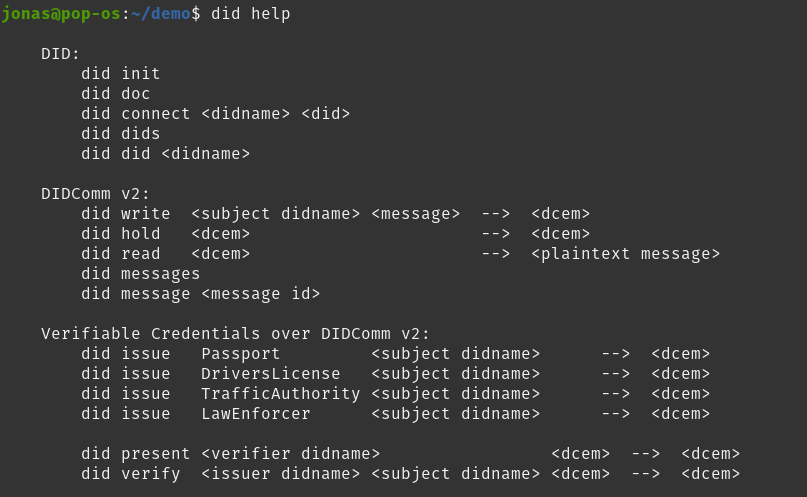
\includegraphics[width=.7\textwidth]{figures/cmd-help.png}
      \caption[]{Example running did help}
    \end{figure}
    
    
    
\subsection{did init}
\begin{itemize}
\item Creates an agent in the current directory.
\item The command creates a new `.did/`-directory, inside your working directory.
\item Your agents DID will be returned to `stdout` when running this command.
\item The command is idempotent.
\item \texttt{did init} bahaves almost identical to \texttt{git init}. This is intentional.
\end{itemize}
    \begin{figure}[htbp]
      \centering
      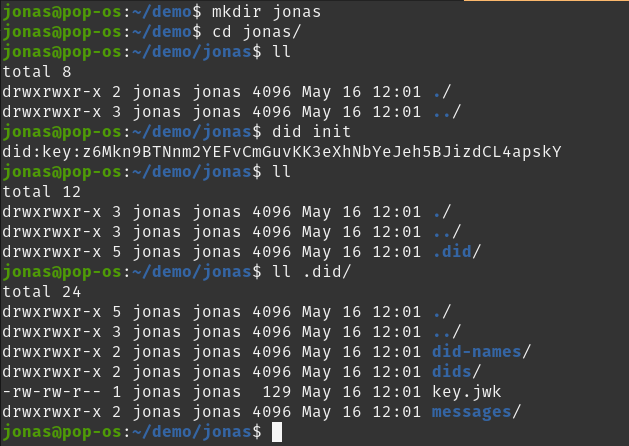
\includegraphics[width=.7\textwidth]{figures/cmd-init.png}
      \caption[]{Example running did init}
    \end{figure}
    


\subsection{did doc}
\begin{itemize}
\item Prints the did-document, controlled by the did agent.
\item Since the did-agent uses did-key as it's underlying did-method, the did-document is generated from the public-private keypair.
\item Another way to describe this is that did-key is self-resolving - the did-document is resolved directly from the did.
\item This is a limitation of the did-key method, and how it is specified.
\item Once created, the did-document pinned to a did-key did, is not possible to edit.
\end{itemize}
    \begin{figure}[htbp]
      \centering
      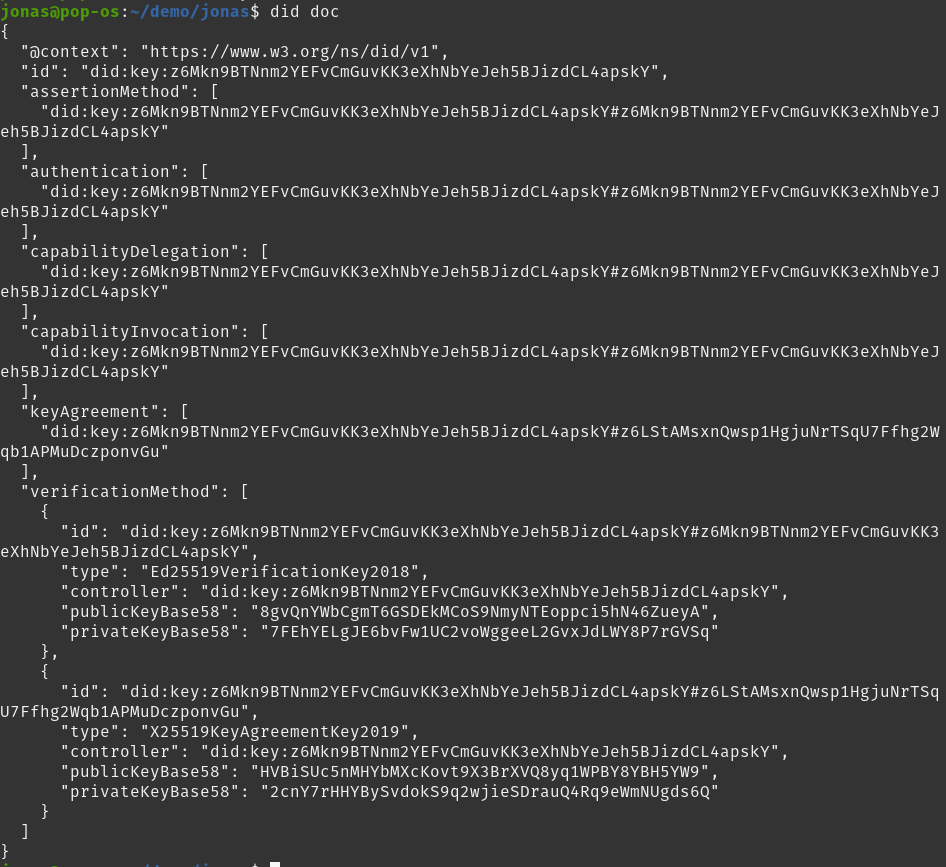
\includegraphics[width=.7\textwidth]{figures/cmd-doc.png}
      \caption[]{Example running did doc}
    \end{figure}



\subsection{did dids}
\begin{itemize}
\item List all dids stored in the agent.
\item Dids are added to the agent when running the `did connect` command.
\end{itemize}
    \begin{figure}[htbp]
      \centering
      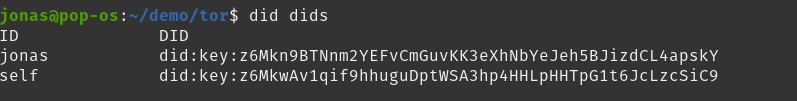
\includegraphics[width=.7\textwidth]{figures/cmd-dids.png}
      \caption[]{Example running did dids}
    \end{figure}



\subsection{did did <didname>}
\begin{itemize}
\item Show the did of a single `<didname>`.
\end{itemize}
    \begin{figure}[htbp]
      \centering
      
\includegraphics[width=.7\textwidth]{figures/cmd-did.png}
      \caption[]{Example running did did}
    \end{figure}



\subsection{did connect <didname> <did>}
\begin{itemize}
\item `did connect` connects a `<didname>` to `<did>`
\item `did connect` gives a `<did>` a `<didname>`.
\item The `<didname>` is used in other commands, as an easy way to refer to another agent's `<did>`.
\end{itemize}
    \begin{figure}[htbp]
      \centering
      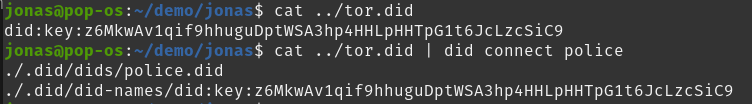
\includegraphics[width=.7\textwidth]{figures/cmd-connect.png}
      \caption[]{Example running did connect}
    \end{figure}



\subsection{did write <didname> <message>}
\begin{itemize}
\item Wraps a user defined message inside a `<dcem>`-envelope.
\item Sets the `to`-header of the `<dcem>` to the underlying `<did>` refered to by the `<didname>`.
\item Gives the message a new globally unique `id`.
\end{itemize}
    \begin{figure}[htbp]
      \centering
      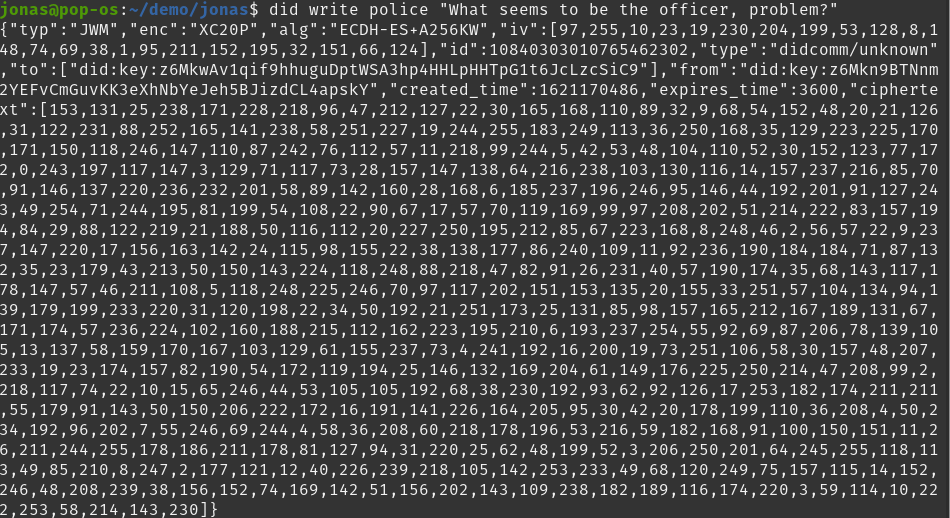
\includegraphics[width=.6\textwidth]{figures/cmd-write.png}
      \caption[]{Example running did write}
    \end{figure}
\newpage

\subsection{did read <dcem>}
\begin{itemize}
\item Unwraps an `<dcem>` message from `stdin` or from `<dcem>`-arg.
\item Prints the plaintext body of the message.
\end{itemize}
    \begin{figure}[htbp]
      \centering
      
\includegraphics[width=.65\textwidth]{figures/cmd-read-message.png}
      \caption[]{Example running did read <message>}
    \end{figure}
    \begin{figure}[htbp]
      \centering
      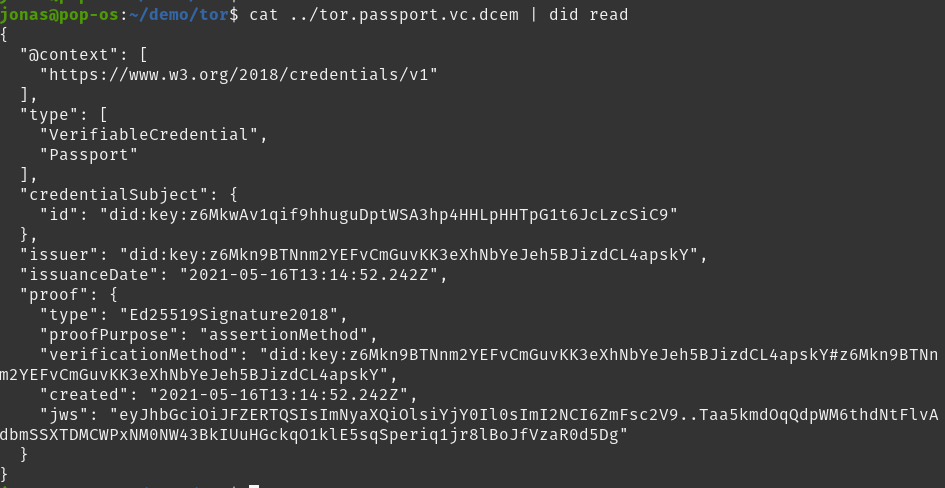
\includegraphics[width=.65\textwidth]{figures/cmd-read-vc.png}
      \caption[]{Example running did read <verifiable credential>}
    \end{figure}
    \begin{figure}[htbp]
      \centering
      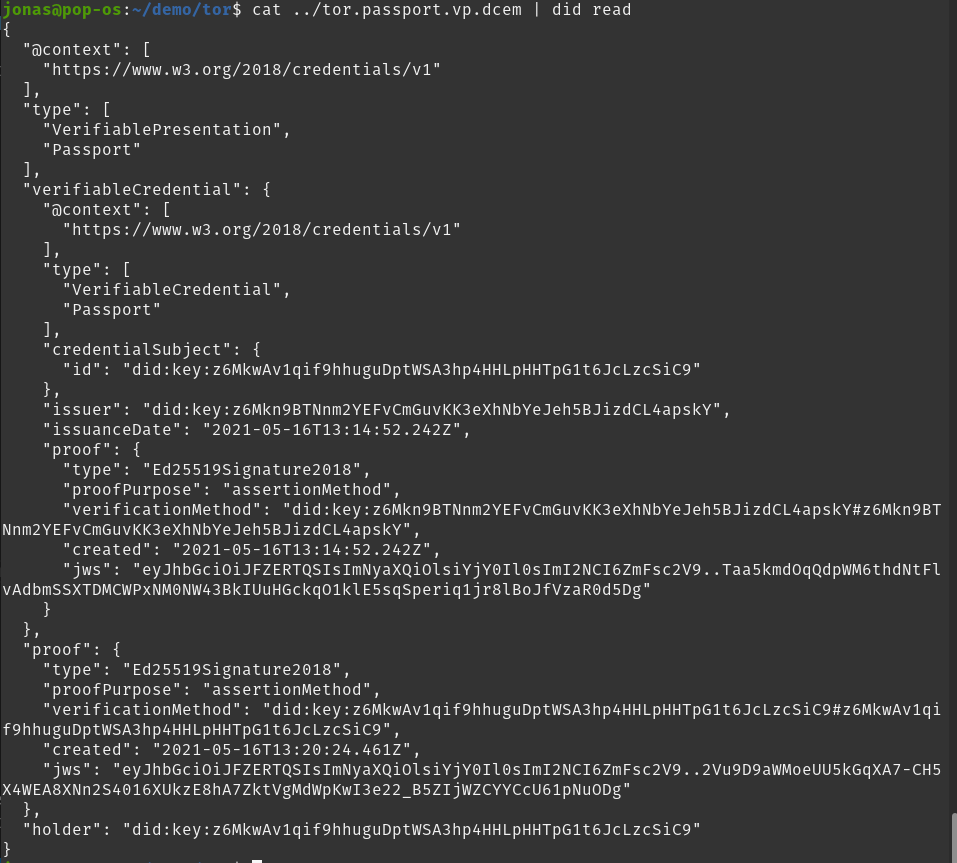
\includegraphics[width=.66\textwidth]{figures/cmd-read-vp.png}
      \caption[]{Example running did read <verifiable presentation>}
    \end{figure}

\newpage



\subsection{did issue <CredentialType> <didname>}
\begin{itemize}
\item Issues a verifiable credential addressed to the `did` of `<didname>`:
\item Issues one of 4 `<CredentialType>`s:
    \begin{itemize}
    \item Passport
    \item DriversLicense
    \item TrafficAuthority
    \item LawEnforcer
    \end{itemize}
\end{itemize}
    \begin{figure}[htbp]
      \centering
      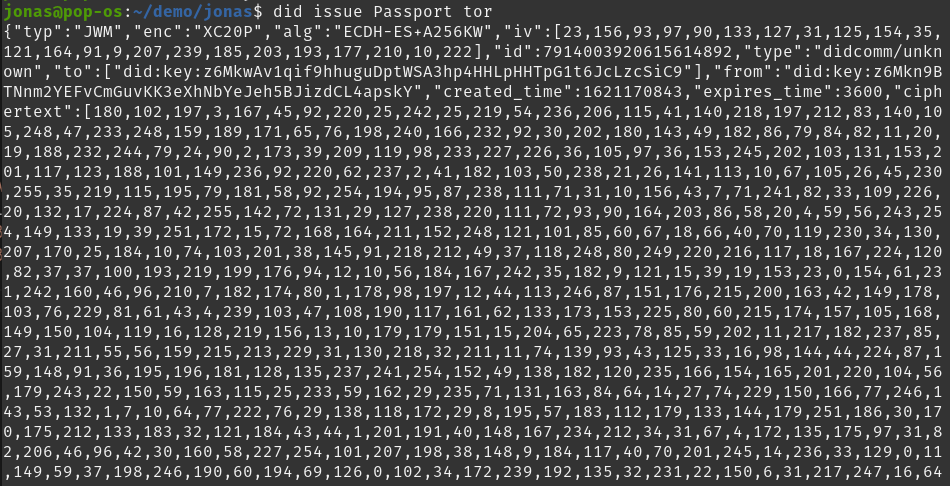
\includegraphics[width=.7\textwidth]{figures/cmd-issue.png}
      \caption[]{Example running did issue}
    \end{figure}



\subsection{did hold <dcem>}
\begin{itemize}
    \item Holds <dcem> and prints it to stdout
\end{itemize}
    \begin{figure}[htbp]
      \centering
      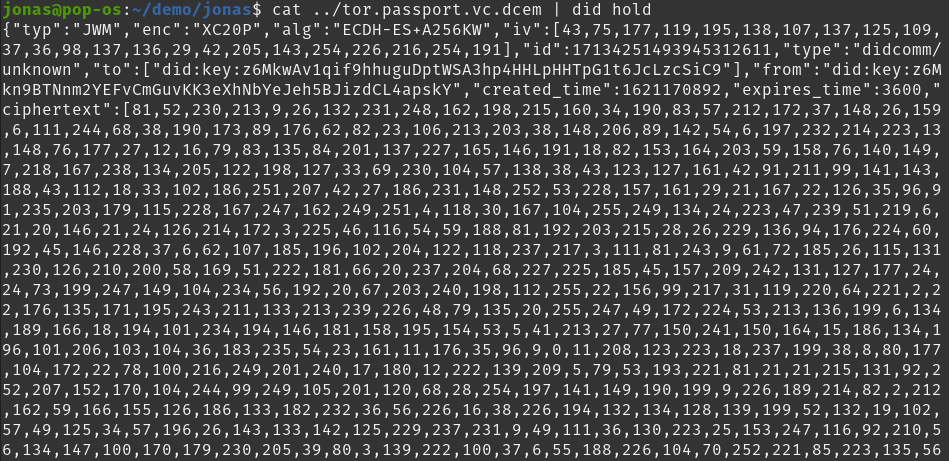
\includegraphics[width=.7\textwidth]{figures/cmd-hold.png}
      \caption[]{Example running did hold}
    \end{figure}

\newpage

\subsection{did present <didname> <dcem>}
\begin{itemize}
    \item Prints a Verifiable Presentation to stdout, with <dcem> as it's content 
\end{itemize}
    \begin{figure}[htbp]
      \centering
      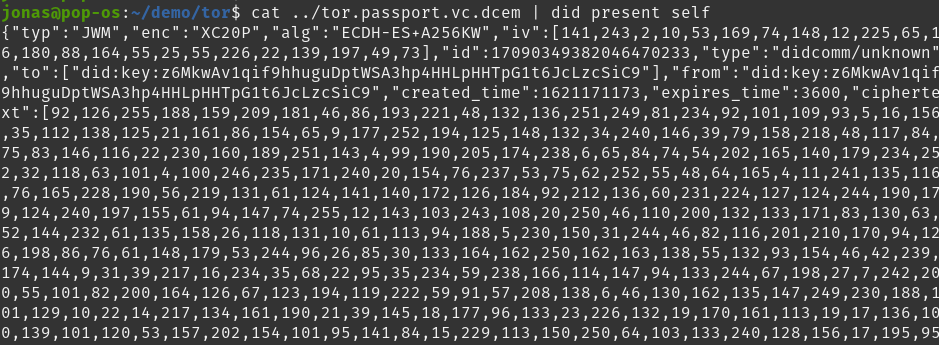
\includegraphics[width=.7\textwidth]{figures/cmd-present.png}
      \caption[]{Example running did present}
    \end{figure}


\subsection{did verify <issuer didname> <subject didname> <dcem>}
\begin{itemize}
\item Prints `<dcem>` to `stdout`, if, and only if, verification succeeds.
\end{itemize}
    \begin{figure}[htbp]
      \centering
      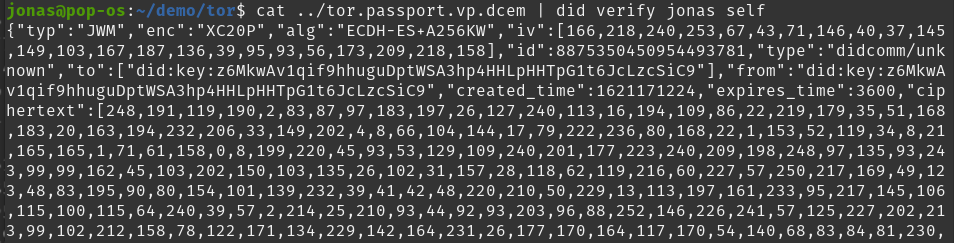
\includegraphics[width=.7\textwidth]{figures/cmd-verify.png}
      \caption[]{Example running did verify}
    \end{figure}
    \begin{figure}[htbp]
      \centering
      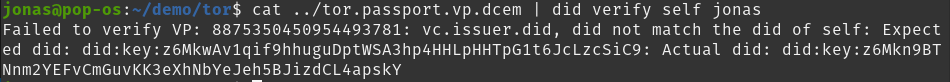
\includegraphics[width=.7\textwidth]{figures/cmd-verify-issuerfails.png}
      \caption[]{Example running did verify when issuer.did fails}
    \end{figure}


\newpage

\subsection{did messages}
\begin{itemize}
\item List all didcomm messages stored in the wallet.
\item Messages are added to the wallet when using the `did hold` command.
\end{itemize}
    \begin{figure}[htbp]
      \centering
      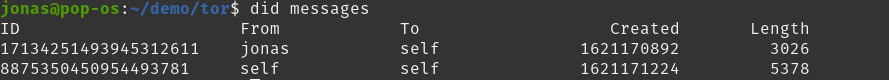
\includegraphics[width=.7\textwidth]{figures/cmd-messages.png}
      \caption[]{Example running did messages}
    \end{figure}

\subsection{did message <message id>}
\begin{itemize}
\item Show the contents of a single didcomm message based on the given `<message id>`.
\end{itemize}
    \begin{figure}[htbp]
      \centering
      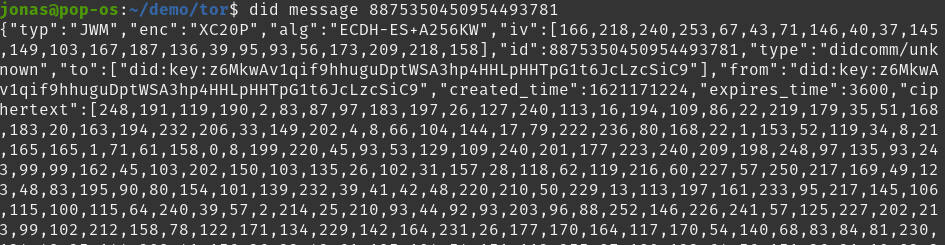
\includegraphics[width=.7\textwidth]{figures/cmd-message.png}
      \caption[]{Example running did message}
    \end{figure}

\section{Intentional limitations of the CLI}

\begin{itemize}
\item None of the commands have any optional-arguments - e.g `--option=<arg>`. This is to keep program logic as simple as possible. If the CLI was intended for a broader audicene with multiple use-cases, options may be added. This CLI is a special purpose CLI, intended to solve a specific use-case, namely the specific proof-of-concept from the problem statement. This is why optional-arguments was not prioritized.
\item Options are much harder to parse correctly than fixed size positional arguments.
\item None of the commands required variable length arguments, which made the implementation easier.
\item None of the commands have filepath arguments. The user is expected to use `cat <filepath>` to read the contents of a file, which is then fed into a positional argument of one of the commands. Example: `did read \$(cat ../message.dcem)` vs `did read ../message.dcem`. This was done to simplify implementation.
\end{itemize}